\documentclass{beamer}
\usetheme{Hannover}


\usepackage{algorithm}
\usepackage{algorithmic}
\usepackage{amsmath}
\usepackage{amssymb}
\usepackage{amsthm}
\usepackage[ngerman,english]{babel}
\usepackage{centernot} 
\usepackage{color}
\usepackage{dsfont}
\usepackage{graphicx}
\usepackage[utf8]{inputenc}
\usepackage{import}
\usepackage{standalone}
\usepackage{qtree}

\usepackage{hyperref}

\title{Integral infeasibility and testing total dual integrality}
\author{David L.Applegate, William Cook S.Thomas McCormick}

\newcommand{\N}{\ensuremath{\mathds{N}}}
\newcommand{\R}{\ensuremath{\mathds{R}}}
\newcommand{\red}[1]{\textcolor{red}{#1}}

\setlength{\itemsep}{-2pt}


\begin{document}

\begin{frame}{Example}
	\begin{enumerate}
		\pause
		\item Item 1:\\
		 $\mathcal{O}(log(n))$ explanation
		\pause
		\item Item 2 
	\end{enumerate}
\end{frame}

%%%%%%%%%%%%%%%%%%
%%%%%%    %%%%%%%%
%%%%%%%%%%%%%%%%%%

\begin{frame}  % important theorems for proofs
	\begin{block}{Complementary Slackness}

		Let $x_0$ and $y_0$ be feasible solutions in the primal and dual problem respectively.
		That is, $Ax_0 \leq b$ and $y_0 A = w; y_0 \geq 0$. \\
		Then $w x_0 = y_0 b$ iff. $(y_0)_i > 0  \rightarrow A_i x_0 = b_i$

	\end{block}	

	\pause

	\begin{block}{Farkas Lemma}

		For $A \in \mathbb{R}^{m \times n}, b \in \mathbb{R}^{m}$ then exactly one of the following is true: \\
		1. There exists $x \in \mathbb{R}^n$ such that $Ax \leq b$ ana $x\geq 0$. \\
		2. There exists $y \in \mathbb{R}^m$ such that $yA=0, yb<0$ and $y \geq 0$. 

	\end{block}

	\pause 

	\begin{block}{Additional note}

		Furthermore note, in relation to Farkas Lemma, we have that exactly one of the following is true: \\
		1. There exists $x \in \mathbb{R}^n$ such that $Ax=b$. \\
		2. There exists $y \in \mathbb{R}^m$ such that $yA=0$ and $by \neq 0$.


	\end{block}

\end{frame}



\begin{frame}
	
	\begin{block}{Hilbert Basis}

		A set of vectors $\{h_1, \dots, h_k\}$ is called Hilbert Basis if each integral vector in the cone $C(\{h_1, \dots, h_k\}) := \{\sum_{i\in \{ 1,\dots,k \}} \lambda_i h_i; \lambda_i \geq 0$ for all $i \in \{1,\dots,k\} \}$ can be written as integral combination of $h_1, \dots, h_k$.

	\end{block}

	\begin{block}{Faces; minimal Faces}

		For $P\subset \mathbb{R}^n$ a polyhedron, $J\subset \{1,\dots , m\}$, define $F_J := \{x \in P | a_i x = b_i$ for $i \in J\}$ as a Face of P.\\
		A minimal Face of $P$ does not contain another Face.

	\end{block}

\end{frame}

\begin{frame}
	\frametitle{Example Faces}
	
	% Beispiel RB Tree
	\begin{figure}[htp]
		\centering
		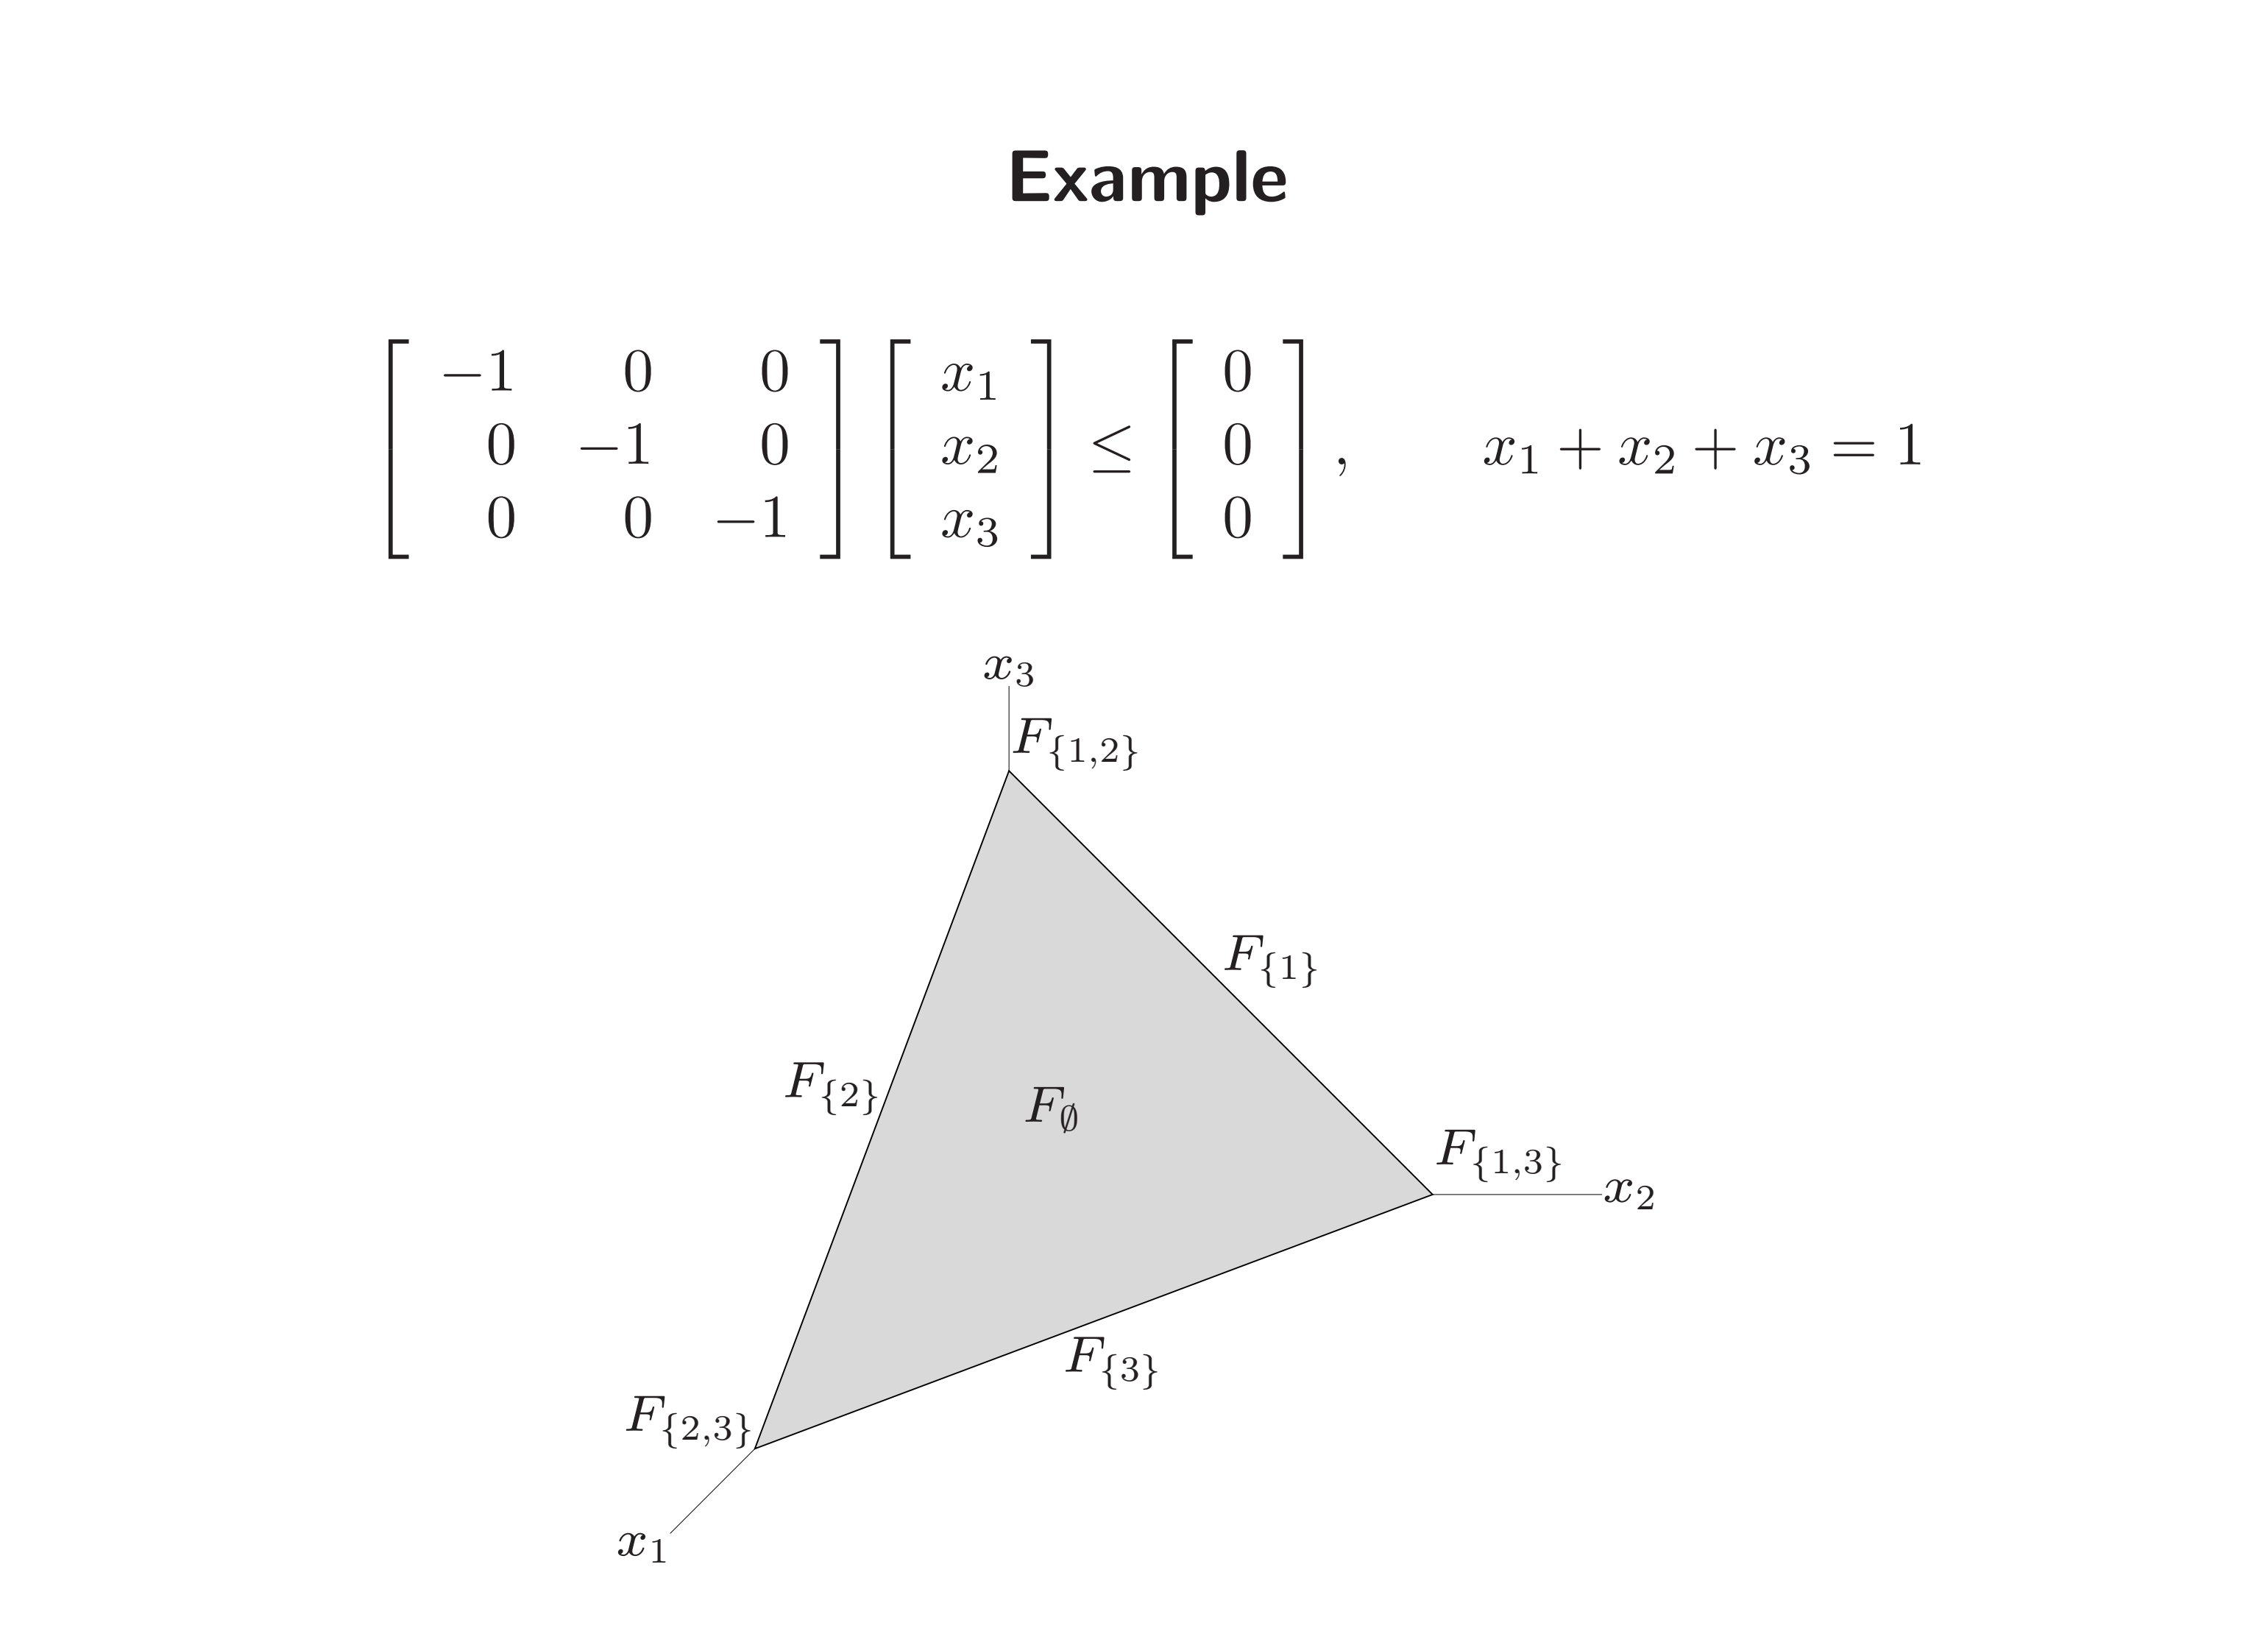
\includegraphics[width=8cm]{images/faces_example.png}
		\caption{http://www.seas.ucla.edu/~vandenbe/ee236a/lectures/polyhedra.pdf}
		\label{fig:faces_example}
	\end{figure}
\end{frame}


%%%%%%%%%%%%%%%%%%
%%%%%%    %%%%%%%%
%%%%%%%%%%%%%%%%%%

\begin{frame}

	\begin{block}{Theorem 1}

		Let $A$ be an integral matrix and $b$ a rational vector such that the linear system $Ax \leq b$ has at least one solution. Then $Ax \leq b$ is totally dual integral if and only if\\

		\begin{itemize}

			\item the rows of $A$ form a Hilbert basis and

			\item for each subset $T$ of inequalities from $Ax\leq b$, if * is infeasible, then this can be proven interally.

		\end{itemize}

	\end{block}

	\begin{block}{Reminder - *}

		For $T\subset \{ 1, \dots, m\}$ * refers to the system with $A_T x= b_T$ and $A_{\overline{T}}x\leq b_{\overline{T}}$.

	\end{block}

\end{frame}


\end{document}
